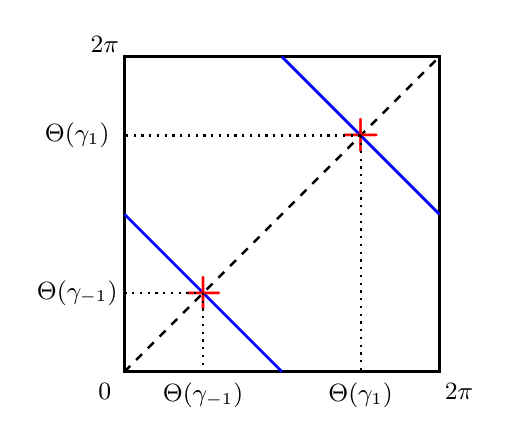
\begin{tikzpicture}[scale=1, every node/.style={font=\small}]
  \def\S{4.0} % side length of the square

  % square [0,1]^2 scaled by S
  \draw[line width=0.9pt] (0,0) rectangle (\S,\S);
    
  % the two diagonal segments (slope -1)
  \draw[blue, line width=1pt] (\S*0.5,0) -- (0,\S*0.5);
  \draw[blue, line width=1pt] (\S, \S*0.5) -- (\S*0.5,\S);

  % dashed diagonal
  \draw[dashed,line width=0.9pt] (0,0) -- (\S,\S);

  % the two X marks
  \node[text=red, font=\bfseries\boldmath, scale=1.6] at (\S*0.25,\S*0.25) {$+$};
  \node[text=red, font=\bfseries\boldmath, scale=1.6] at (\S*0.75,\S*0.75) {$+$};

  \draw[dotted, line width=0.8pt] (\S*0.25, \S*0.25) -- (\S*0.25, 0);
  \node at (\S*0.25,-0.3) {$\Theta(\gamma_{-1})$};
  \draw[dotted, line width=0.8pt] (0, \S*0.25) -- (\S*0.25, \S*0.25);
  \node at (-0.6,\S*0.25) {$\Theta(\gamma_{-1})$};
  \draw[dotted, line width=0.8pt] (\S*0.75, \S*0.75) -- (\S*0.75, 0);
  \node at (\S*0.75,-0.3) {$\Theta(\gamma_{1})$};
  \draw[dotted, line width=0.8pt] (\S*0.75, \S*0.75) -- (0, \S*0.75);
  \node at (-0.6,\S*0.75) {$\Theta(\gamma_{1})$};

  % corner labels 0 and 2pi like your sketch
  \node at (-0.25,-0.25) {$0$};
  \node at (\S+0.25,-0.25) {$2\pi$};
  \node at (-0.25,\S+0.15) {$2\pi$};

\end{tikzpicture}
